%% introduction.tex
%%

%% ==============================
\chapter{Introduction}
\label{ch:Introduction}
%% ==============================
	Ever since the beginning of the \nth{19} century science in general but especially the field of physics has been undergoing an unbelievably quick and vast development. The possibilities arising from automated analysis through the use of advanced computation grids connected to the optimization of manufacturing processes for detectors leave the world - and even scientist - amazed. Nevertheless, with more and more phenomena well understood, the remaining tasks often require huge projects and large collaborations. One of these projects, and a magnificent one at that, is the KATRIN experiment.
	Working on the project is a liaison of 15 universities and research facilities with over 150 coworkers aspiring to find the absolute neutrino mass scale. So at first, a introduction covering the postulation and discovery of the neutrino as well as latest results from research is given.
	\\
	Another important topic for this thesis are cosmic rays: Both the particle most significant for KATRIN, the neutrino, and the background inducing muon are generated in different interactions with the atmosphere. That is why a part of this introduction will be devoted to the description of air showers.
	
	\section{Neutrinos - the early years}
	\label{ch:Introduction:sec:Neutrino-theEarlyYears}
	The neutrino was not discovered in the conventional meaning but postulated by Wolfgang Pauli, then under the name of ``neutron'', as a explanation for the spectrum of the beta decay showing a continous energy distribution which did not concur with the idea of a two body decay \cite{fermi}. 
	\begin{equation}
		\ce{p -> n + e^-}
	\end{equation}
	Coservation laws of energy, momentum and angular momentum were violated.
	The neutrino solved this problem by being a carrier of different kinetic energies thus allowing for a continuous spectrum.
	\begin{equation}
		\ce{p -> n + e^- + \bar\nu_e}
	\end{equation}
	To be compliant with the laws of conversation, the new particle needed to be of spin 1/2 and chargeless.
	The first experimental evidence for this particle was then given by Cowan and Reines \cite{neutrinoEvidence} who observed the reaction of electron-anti-neutrinos and free protons in the large neutrino flux of a nearby nuclear reactor.
	\begin{equation}
		\ce{\bar\nu_e + p -> e^+ + n}
	\end{equation}
	They then looked for two events: a pair of \SI{511}{\kilo\electronvolt} photons from electron-positron annihilation as well as the $\gamma$ from neutron capture some \SI{}{\micro\second} afterwards.
	Following the electron neutrino, both other known neutrino generations have been attested for in various experiments, the first ones to find evidence for $\nu_\mu$ and $\nu_\tau$ were to be Danby and Gaillard \cite{muNeutrino} and the DONUT experiment \cite{tauNeutrino} respectively.\\

	
	\section{Neutrino sources}
	\label{ch:Introduction:sec:neutrinoSources}
	Next to the first indicator of neutrinos, the beta decay with its continuous spectrum, many other reactions produce neutrinos besides easily detectable products. An overview over natural sources creating the largest flux through earth as well as experimental sources is given below, figure 
	\begin{figure}
		\begin{minipage}{0.65\textwidth}
			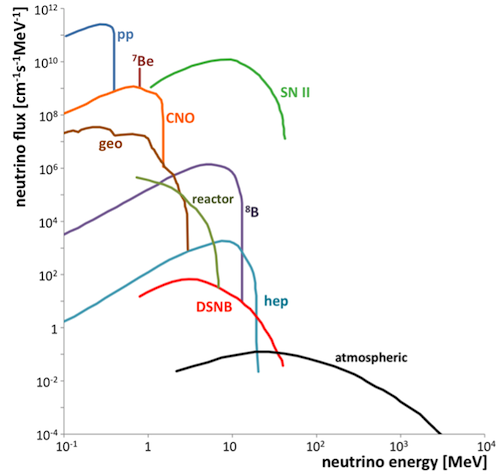
\includegraphics[width=\textwidth]{graphics/neutrinos/neutrinoSpectrum.png}
		\end{minipage}
		\begin{minipage}{0.34\textwidth}
		\caption[Neutrino sources]{~}A graph for different neutrino sources both natural and artificial. In the upper left, solar reactions creating a large integral flux. In the upper mid, the supernovae type II. Peaking at around $10^5$ \SI{}{\per\second} \SI{}{\per\square\centi\meter\per\mega\electronvolt}, geoneutrinos. Right of it reactor neutrinos and $^8$B, the $\beta^+$ decaying boron isotope. Following below are the diffuse super novae background, another solar reaction, hep, and, last and least, the atmospheric neutrinos.
		\label{fig:neutrinos:neutrinoSources}	
		\end{minipage}

		
	\end{figure}

	\begin{itemize}
	\item {\bf Primordial neutrinos}\\
		Lingering around since the ``Big Bang'', neutrinos with rather low, thermal energies form a cosmic neutrino background at $T_\nu\approx \SI{1.95}{\kelvin}$. These neutrinos discoupled shortly after the Big Bang when densities rapidly dropped and with it the weak force's reaction rate that before kept an equilibrium between protons, neutrons electrons and neutrinos. This process of ``freezing out'' alone leads to a static number density of \SI{336}{\per\cubic\centi\meter} for the sum over all three neutrino flavors.
	\item {\bf Supernovae neutrinos}
		Supernovae type II, which occur less often than the type I and only in stars with $M> 8M_\odot$, are known to produce large quantities of neutrinos. Inside the burned out collapsing star, the electrons' degeneracy pressure leads to de-leptonization of the core by electron capture.
		\begin{equation}
			\ce{e- + p -> n + \nu_e}
		\end{equation}
		This process produces high energy neutrinos leaving the core and carrying away energy in the process - and large quantities of that: about \SI{99}{\percent} of the energy released during a type II supernova cooling phase is carried away by neutrinos.

	\item {\bf Solar neutrinos}\\
		Our sun's $pp$ reaction chain equation (\ref{ppChain}) - dominant in its energy production - produces neutrinos in a continuous energy range (upper energy limit given) together with other, less dominant reactions.
		\begin{align}
		\label{ppChain}
			\ce{^1H + ^1 H} & \ce{ -> ^2 He + e+ + \nu_e} && (\SI{0.42}{\mega\electronvolt})\\
			\ce{^8B } & \ce{-> ^8Be + e+ + \nu_e} && (\SI{14.06}{\mega\electronvolt})\\
			\ce{^3He + p } & \ce{ -> ^4He + e+ + \nu_e} && (\SI{18.77}{\mega\electronvolt})
		\end{align}

		Further on, electron capture processes add line spectra to the picture
		\begin{align}
			\label{eq:Berillium}
			\ce{^7Be + e-} & \ce{-> ^7Li + \nu_e}\\
			\ce{^1H + ^1H + e-} & \ce{-> ^2H + \nu_e} (\SI{1.55}{\mega\electronvolt})
		\end{align}
		where $^7$Be emits at two energies: mostly at \SI{0.86}{\mega\electronvolt}(\SI{90}{\percent}) and another, lower energy line at \SI{0.38}{\mega\electronvolt} (\SI{10}{\percent}) \cite{bethgeKernphysik}.
		These reactions are responsible for the largest part of the solar neutrino flux through the earth. Predictions on this flux are shown in figure \ref{fig:neutrinos:solarNeutrinos} together with other model calculations on flux expectations.
		Solar neutrinos were essential for oscillation research and by that for the proof that neutrinos are in fact massive (see chapter \ref{ch:Introduction:sec:neutrino Oscillations}).
		\begin{figure}
		\centering
			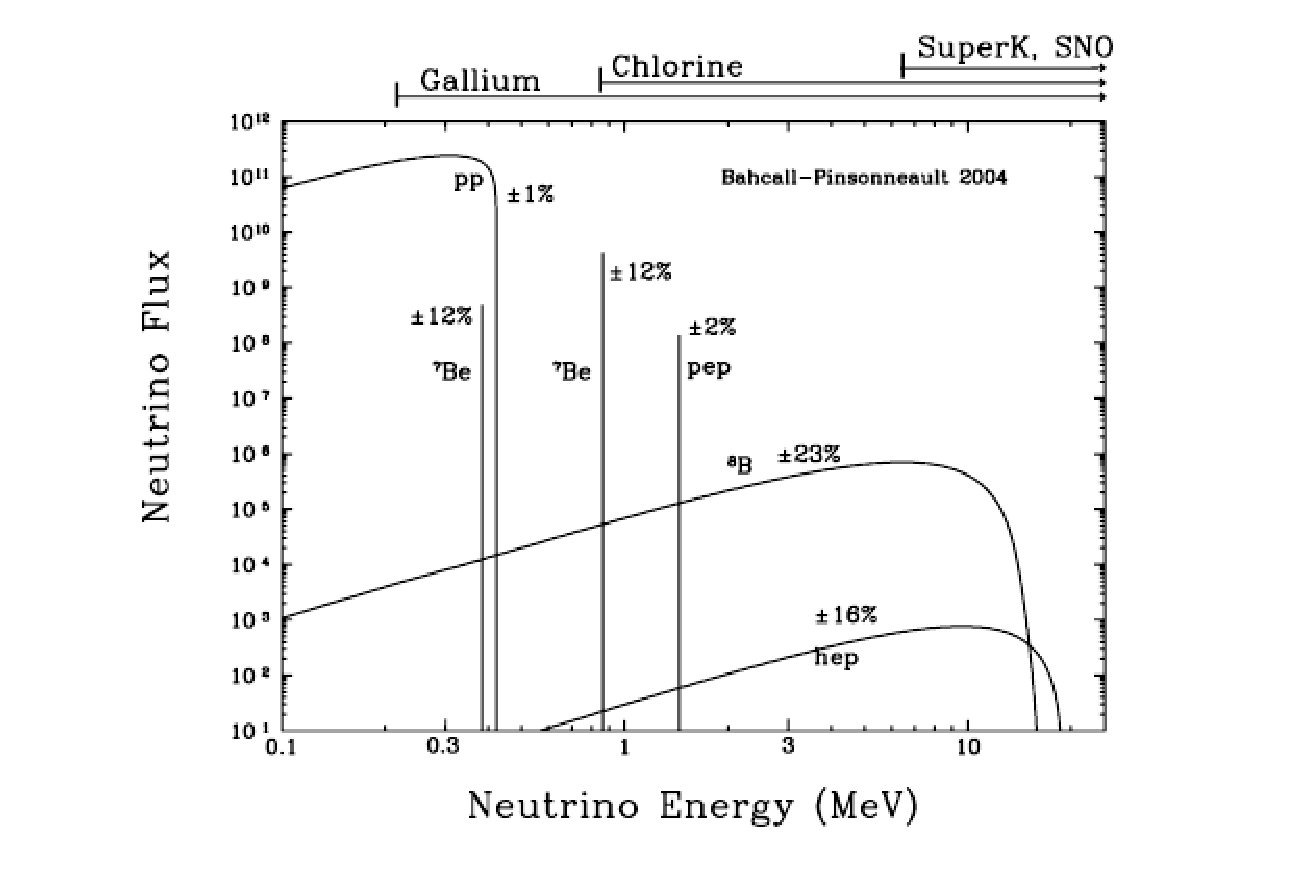
\includegraphics[width=0.8\textwidth]{graphics/neutrinos/solarNeutrinos.eps}
			\caption[Solar neutrino Flux]{The graph shows the theoretical solar neutrino flux in \SI{}{\per\square\centi\meter \per\second \per\mega\electronvolt} over the neutrino energy - for line sources in \SI{}{\per\square\centi\meter \per\second}. Different processes are shown, the dominant pp process is visible in the upper left. CNO fluxes are dropped in this figure. On the very top, the sensitivities of different experiments are shown.}
			\label{fig:neutrinos:solarNeutrinos}
		\end{figure}

	\item {\bf Atmospheric neutrinos}\\
		As described in section \ref{ch:Introduction:sec:Cosmic Air Showers} cosmic rays, consisting mostly of hadrons, which, in turn, are mostly protons, constantly impact onto the upper layers of the atmosphere. Here, they create air showers, cascades of the initially high energy particles into thousands of particles of lower energies. In that process, not only muons relevant considering background processes in KATRIN, but also neutrinos originate raising the flux through earth.
	\item {\bf Reactor neutrinos}\\
		Nuclear fission produces large quantities of neutrons that decay following 
		\begin{equation}
			\ce{n -> p + e- + \bar\nu_e}
		\end{equation}

		A fission reactor, in which many of these reactions concur, is hence a strong source of neutrinos, depending on the reactor's size of course. On an average \SI{}{\giga\watt} reactor, around 6 neutrinos per fission reaction emerge. These sources are used in many experiments, among other things to prove the existence of neutrino oscillations (see chapter \ref{ch:Introduction:sec:Massive neutrino:subsec:neutrino Oscillations}). The Daya Bay experiment for example was able to attest the disapperance of $\bar\nu_e$ in a baseline experiment \cite{dayaBay}.
	\item {\bf Neutrinos from $\beta$ decays}\\
		Very important for the KATRIN experiment are neutrinos from beta decays, more precisely the tritium beta decay. This is described in more detail in chapter \ref{ch:The KATRIN experiment:sec:Measurement Principle}.
	\end{itemize}

	
	
    \section{Neutrinos in the standard model}
    \label{ch:Introduction:sec:Neutrinos in the standard model}
    During the second part of the 20th century, a model stating 16 particles has been developed to describe a huge portion of known phenomena - the standard model. It contains six quarks and six leptons (both made up of three particle generations) making up the matter as well as four types of Gauge Bosons. The latter are carriers of the standard model's interactions of the former particles, meaning all interactions of matter are based on the exchange of one or more of the Gauge Bosons.
    Lately, proof for the Higgs particle, a scalar boson, stated as a carrier of mass seems to have been found at CERN \cite{CMS, ATLAS}. It is the last particle to complete the standard model.
    For our universe, gravity, the graviton generated force, plays a major role for formation and stability of almost all larger structures. In particle physics however, it can mostly be neglected. Here, only the strong and weak as well as the electromagnetic interaction make for noticeable contributions to phenomena observed. That is why, in the standard model, gravity as well as its carrier, the graviton, are disregarded.
    \begin{figure}
    	\centering
    	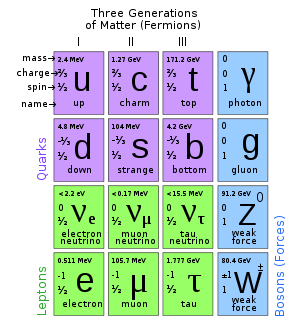
\includegraphics[width = 0.6\textwidth]{graphics/standardModel/particles.png}
    	\caption[standard model particles]{Particles stated in the standard model. On the upper left quarks, on the lower left leptonic particles. The very right row contains the bosonic force particles. Note the absence of the graviton.\cite{particlesSM}}
    	\label{fig:standardModel:particles}
    \end{figure}
	
    Most of what we can observe with our bare eyes or in basic experiments is attributable to the electromagnetic force or gravity, however, strong and weak interaction do play a major role when it comes to high energy physics. Here, the limited reach of the two is overcome by small distances between interacting particles. In case of the neutrino, detection and by that the study of its characteristics is even more difficult as it interacts only gravitationally and weakly. Now, as mentioned before, gravity is indeed long range, but very weak in force. And although weak intraction is a lot stronger compared to gravity, it is still weak compared to both electromagnetic and strong interactions. That is why the neutrino is considered elusive, detection efficiencies are low and only large scale detectors are able to detect statistically relevant amounts of neutrinos.
    One method used quite frequently is the Cherenkov radiation emitted by particles travelling through matter at speeds above the speed of light. The occuring cones of light, comparable to the supersonic cones planes cause in air, can be detected by standard photomiltiplier tubes. The problem is that, as mentioned above, the volumes to be able to make dependable statements on directions and energies need to be large. This is why most experiments make use of ``natural'' detectors such as water \cite{Antares} or even ice \cite{iceCube}.
    Other approaches are to catch neutrinos in reactions where those are required such as inverse beta decays in reactors
    \begin{equation}
		\ce{\bar\nu_e + p -> e^+ + n}.
    \end{equation}
   
    
    In the standard model, neutrinos are considered massless. 
    Many experiments though have shown that the weightless neutrino is a wrong assumption. Most of these were experiments proving neutrino oscillations with both reactor neutrinos and solar neutrinos such as Kamiokande\cite{PhysRevLett.110.181802}, the Daya Bay experiment \cite{dayaBay2} or SNO \cite{SNOOscillations}.
    Important for those experiments is the known source location making baseline analysis possible.
    
    Up till now, only the differences of the squared masses are known. This leads to different relations depending on how masses are distributed between the flavors, see figure \ref{fig:massSchemes}, and how large they are absolutely, see figure \ref{fig:massHierarchy}. This problem is solved by the knowledge of one of the masses. KATRIN is on the verge of finding the $\nu_e$'s mass. Two mass schemes are possible: the normal and the inverted one. Normal means that the smallest number also describes the smallest mass state, i.e. $m_{\nu_1} < m_{\nu_2} < m_{\nu_3}$. In the inverted scheme, the squared mass difference of eigenstates two and three is not directed upwards, but pushes the $m_{\nu_3}$ mass below the other two.
    
    \begin{figure}
    \centering
    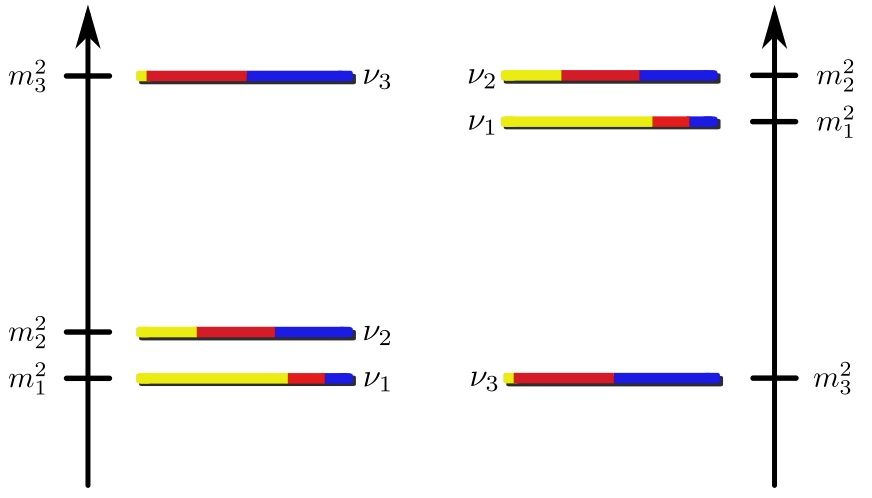
\includegraphics[width=0.7\textwidth]{graphics/standardModel/massHierarchy.jpg}
    	 \caption[Neutrino mass hierarchy]{The possible mass hierarchies for neutrinos. Left, the normal scheme with $m_{\nu_1} < m_{\nu_2} < m_{\nu_3}$, on the right the normal scheme where $m_{\nu_1} < m_{\nu_2}$ is still true, though both $m_{\nu_3} < m_{\nu_1}$ and $m_{\nu_3} < m_{\nu_2}$. The colored bars represent the matrix elements for each flavor, i.e. the probabilities of measuring the mass eigenstate while detecting a pure flavor. Yellow stands for $\nu_e$, red for $\nu_\mu$ and blue for $\nu_\tau$.}
    	\label{fig:massSchemes}
    \end{figure}
    \begin{figure}
    \centering
    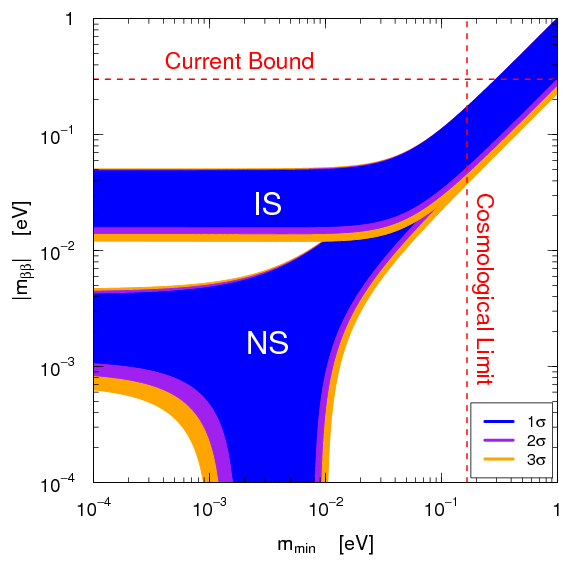
\includegraphics[width = 0.7 \textwidth]{graphics/standardModel/massSchemes.png}
	\caption[Effective neutrino mass]{The possible effective masses for neutrinos depending on the lightest neutrino mass $m_{min}$ shown on the x-axis. Normal and inverted scheme are marked NS and IS. The current bound from $0\nu\beta\beta$ decay is displayed as well as cosmological limitations. }
    	\label{fig:massHierarchy}
    \end{figure}

    
    \section{Neutrino Oscillations}
    \label{ch:Introduction:sec:neutrino Oscillations}
      If the neutrinos were without mass, its mass eigenstates would equal its flavor eigenstates.
    First doubts concerning this assumptions occurred as inconsistencies between the measured and the calculated solar $\nu$-flux occurred at the Homestake mines \cite{homestake}. As the count on $\nu_e$ was too low, the theory of neutrino oscillations emerged, stating that a mixture of flavors was possible as the flavors were made up of all three of the mass eigenstates. The mixture is described by the so called Pontecorvo-Maki-Nakagawa-Sakata matrix:
        \begin{equation}
        \left(
        \begin{array}{c}
	  |\nu_e>\\
	  |\nu_\mu>\\
	  |\nu_\tau>\\
        \end{array}
        \right)
	 = \left(
	\begin{array}{ccc}
      	U^*_{e,1} & U^*_{e,2} & U^*_{e,3}\\
      	U^*_{\mu,1} & U^*_{\mu,2} & U^*_{\mu,3}\\
      	U^*_{\tau,1} & U^*_{\tau,2} & U^*_{\tau,3}\\
      	\end{array}
	\right)
	\left(
	\begin{array}{c}
      	|\nu_1>\\
      	|\nu_2>\\
      	|\nu_3>\\
    	 \end{array}
    	 \right)
    \end{equation}
    In this equation, the matrix U can be parametrized through a combination of three rotation matrices and a complex phase factor $\delta_D$ as well as two complex majorana phases $\delta_M$
    
    \begin{equation}
	\centering
	\begin{split}
     U = \left(
	\begin{array}{ccc}
      	1 & 0 & 0\\
      	0 & c_{23} & s_{23}\\
      	0 & -s_{23} & c_{23}\\
   	\end{array}
	\right)
	\left(
	\begin{array}{ccc}
      	c_{13} & 0 & s_{13}e^{-i\delta_D}\\
      	0 & 1 & 0\\
      	-s_{13}e^{-i\delta_D} & 0 & c_{13}\\
      	\end{array}
	\right)\cdot\\
	\cdot\left(
	\begin{array}{ccc}
      	c_{12} & s_{12} & 0\\
      	-s_{12} & c_{12} & 0\\
      	0 & 0 & 1\\
      	\end{array}
	\right)
		\left(
	\begin{array}{ccc}
      	e^{i\delta_{M1}} & 0 & 0\\
      	0 & e^{i\delta_{M2}} & 0\\
      	0 & 0 & 1\\
      	\end{array}
	\right)
	\end{split}
    \end{equation}
    where $c_{ij}=\cos{\theta_{ij}}$ and $s_{ij}=\sin{\theta_{ij}}$.\\
	Now the pure eigenstate of a neutrino for t=0 can be described by three matrix elements and the corresponding mass eigenstates.
	\begin{equation}
		\left|\nu(t=0)\right> = \left|\nu_\alpha\right> = U^*_{\alpha1} \left|\nu_1\right> + U^*_{\alpha2} \left|\nu_2\right> + U^*_{\alpha3} \left|\nu_3\right> 
	\end{equation}
	The time evolution of this state now reveals the oscillations of the neutrino from flavor to flavor, as the time evoluted states are not flavor eigenstates for every point in time. 
	\begin{equation}
		\left|\nu_\alpha(t>0)\right> = U^*_{\alpha1} e^{-iE_{\alpha1}t}\left|\nu_1\right> + U^*_{\alpha2} e^{-iE_{\alpha2}t}\left|\nu_2\right> + U^*_{\alpha3}e^{-iE_{\alpha3}t} \left|\nu_3\right> \neq \left|\nu_\alpha\right> 
	\end{equation}
	This means that the probability to find a state different from the initial one is non-zero for most times.
	\begin{equation}
		\begin{split}
			\left|\nu_\alpha(t)\right> = \sum_{k = 1,2,3} U^*_{\alpha k}\exp\left(-iE_k t\right)\left|\nu_k\right>
		\end{split}
	\end{equation}
	for every state $\left|\nu_\alpha\right>$. If the mass eigenstates in turn are expressed as a mixture of flavor eigenstates, one can extract the prefactor of the sums components as the transition probability for each single flavor:
	\begin{equation}
		P(\nu_\alpha \rightarrow\nu_\beta) = \left| \left<\nu_\beta\right|\left.\nu_\alpha(t)\right>\right|= \left|\sum_{k=1,2,3}U^*_{\alpha k} \exp{\left(-iE_kt\right)}U_{\beta k}\right|^2
	\end{equation}
	Various baseline experiments have found results for all mixing angles except $\Theta_{23}$ for which a lower limit is known according to \cite{reviewOfParticlePhysics}
	\begin{table}
	\centering
		\begin{tabular}{|c|c|}
		\hline
			parameter & value\\
			\hline			
			$\sin^2{\left(2\Theta_{12}\right)}$& \SI{0.875\pm 0.024}{}\\
			$\Delta {m^2}_{21}$&\SI{7.5 \pm 0.20 e -5}{\square\electronvolt}\\
			$\sin^2{\left(2\Theta_{23}\right)}$& >\SI{0.95}{}\\
			$\Delta {m^2}_{32}$ & \SI{2.32(12)}{\square\electronvolt} \\
			$\sin^2{\left(2\Theta_{13}\right)}$ & \SI{0.095\pm0.010}{}\\
			\hline
		\end{tabular}
		\caption[Neutrino parameters]{Given are the latest known mixing angles and squared mass differences. For $\sin^2{\left(2\Theta_{23}\right)}$, the lower limit is given.}
		Though mixing angles are known pretty well, there are still experiments being built that challenge the current error margins such as the LENA experiment which might be able to raise the precision of the mixing angle $\Theta_{12}$ by a factor of 10 and  may even find the still unknown mixing angle $\Theta_{13}$ (\cite{LENA}).
		\label{tab:neutrinoParameters}
	\end{table}
	
	    \section{Indirect measurement of neutrino mass}
    \label{ch:Introduction:sec:Massive neutrino:subsec:indirect Neutrino Mass measurement}
   	One approach to get access to the neutrino mass is on indirect ways, i.e. using data that is affected by neutrinos but does not directly involve them. Two main techniques are to be indicated here.\\\\
   	First, the search for neutrinoless double beta decay, $0\nu\beta\beta$. The double beta decay $2\nu\beta\beta$ in which two neutrinos are emitted only occurs if the single $\beta$ decay is prohibited by a heavier $^A_{Z+1}X$ core and follows the equation
   	\begin{equation}
   		\ce{^A_ZX -> ^A_{Z+2}X + 2 e- + 2 \bar\nu_e}.
   	\end{equation}
	Compared to this $2\nu\beta\beta$ decay the $0\nu\beta\beta$ decay can exist only if the neutrino is its own anti-particle, a so called Majorana neutrino. Then, if a nucleus double beta decays, the neutrino from one vertex can be absorbed in the second as an anti-neutrino with inversed helicity - or vice versa. As this change in helicity is only possible for a massive particle, the $0\nu\beta\beta$ decay would be further proof of a massive neutrino. Furthermore, as the probability for a helicity change is correlated to particle mass the rate, and with it the half life $t_{1/2}$, would depend on the effective Majorana neutrino mass square \cite{currentNeutrinoSearches}.
    \begin{equation}
    	\Gamma_{0\nu\beta\beta} \propto \left| \sum{U_{ei}^2m\left(\nu_i\right)}\right|^2
    \end{equation}
    
    Secondly, the problem can be approached by calculations using astrophysical data.\\
    For one, the formation of galaxies and other structures in the universe depends on the neutrino mass. In the formation, neutrinos wash out the structures as they act as hot dark matter. A galaxy's power spectrum's fluctuation is supressed by massive neutrinos. Using long term spectroscopic galaxy surveys like SDSS\cite{SDSS} or studying the cosmic microwave background like WMAP \cite{WMAP} or Planck \cite{Planck}, a upper limit of \SI{0.6}{\electronvolt} on $\sum_\nu m_\nu$ can be given.\\
    As the indirect methods for neutrino mass measurements depend at least to some point on model assumptions, the direct methods in the next section play a key role in finding standalone values or limits for neutrino mass.

    
    \section{Direct measurement of neutrino mass}
    \label{ch:Introduction:sec:Massive neutrino:subsec:direct Neutrino Mass measurement}
    Direct measurements of the neutrino mass require a reaction known to include neutrinos in its equation, usually the previously mentioned $\beta$ decay. Advantageous for direct measurements is the only assumption made is the applicability of the relativistic energy-momentum-relation $E^2 = m^2c^4 + p^2c^2$. This makes the results mostly model independent. There are both spectrometric and calorimetric approaches. While the scale of spectrometers is getting bigger and bigger, calorimetric approaches seem to be a reasonable alternative, although the slow detector response - the detector material itself is decaying - requires for large arrays of detectors leading to extensive space requirements as well at some point. The luminosity of spectrometer experiments though is unachieved by any other. That is why the KATRIN collaboration is working on a setup to measure electrons from Tritium decay to determine the neutrino mass. 
    Tritium is advantageous for several reasons listed below.
    \begin{itemize}
    	\item A high luminosity is ensured by the short half life of $t_{1/2} = \SI{12.3}{\year}$. This makes small amounts of the emitter sufficient to ensure good statistical results.
    	\item At the same time, the inverse of the cubic endpoint energy ($1/E_0^3$) defines the amount of electrons emitted in the endpoint region (up to \SI {1}{\electronvolt} below the endpoint). Tritium's low endpoint energy of \SI{18.6}{\kilo\electronvolt}, undercut only by one $\beta$ emitter, rhenium, that has other disadvantages, ensures high luminosity at the detector.
    	\item According to \cite{superallowance}, as the tritium beta decay is superallowed , the matrix element $\left|M_{had}\right|$ is energy independent making corrective energy calculations unnecessary. This simplifies analysis procedures.
    	\item Another simplification compared to different emitters is the easily calculable electron shell configuration. Excited states and their energies are accessible in theory for all decaying particles.
    	\item As far as scattering is concerned, tritium is a well suited material as well. Its low atomic number makes for small cross sections for inelastic scattering. This reduces energy smearing inside the source volume.
    \end{itemize}
    These reasons make tritium the element of choice for KATRIN.\\\\
    The above mentioned rhenium is used in the calorimetric approach. Experiments like MARE \cite{MARE2007} use rhenium in bolometers as both emitter and detector. The lower endpoint energy of \SI{2.47}{\kilo\electronvolt} guarantees a rather big fraction of electrons with energies near the endpoint, but this is largely compensated for by the much longer half life of $t_{1/2} = $\SI{4.32 e 10}{\year}. Still, the mass of rhenium required to gain statistically relevant results remains below the tritium mass used in KATRIN. The MARE strategy is to split the radioactive material and use it in many small microbolometers. That is benefitial as readout is slow and the rate per bolometer is reduced by lowering the emitter mass. Thermistors then sample the temperature catching peaks induced by electrons from $\beta$ decays scattering inside the solid source.
    The experiment set up by the Milano collaboration has set upper limits of
    \begin{equation}
    	m_{\bar\nu_e} < \SI{15}{\electronvolt} ~ {\rm at}~ \SI{90}{\percent\CL}.
    \end{equation}
    This limit shall be pushed to \SI{0.2}{\electronvolt} according to \cite{MARE2007}.  

	\section{Cosmic rays from the viewpoint of KATRIN}
    \label{ch:Introduction:sec:Cosmic Air Showers}
    When high energy particles hit the upper parts of the atmosphere, a cascade of particles generated from the interaction with atmospheric molecules and atoms follows. Most primary particles are nucleons, most of which again are free protons (85\%), i.e. Hydrogen ions, followed by $\alpha$ particles (15\%). Helium nucleons' fluxes are already about an order of magnitude below the hydrogen ones, higher mass number nuclei show even lower rates, see figure \ref{fig:Introduction:sec:CosmicRays} \cite{highEnergyCosmicRays}.
    \begin{figure}
	\begin{minipage}[d]{0.49 \textwidth}
		  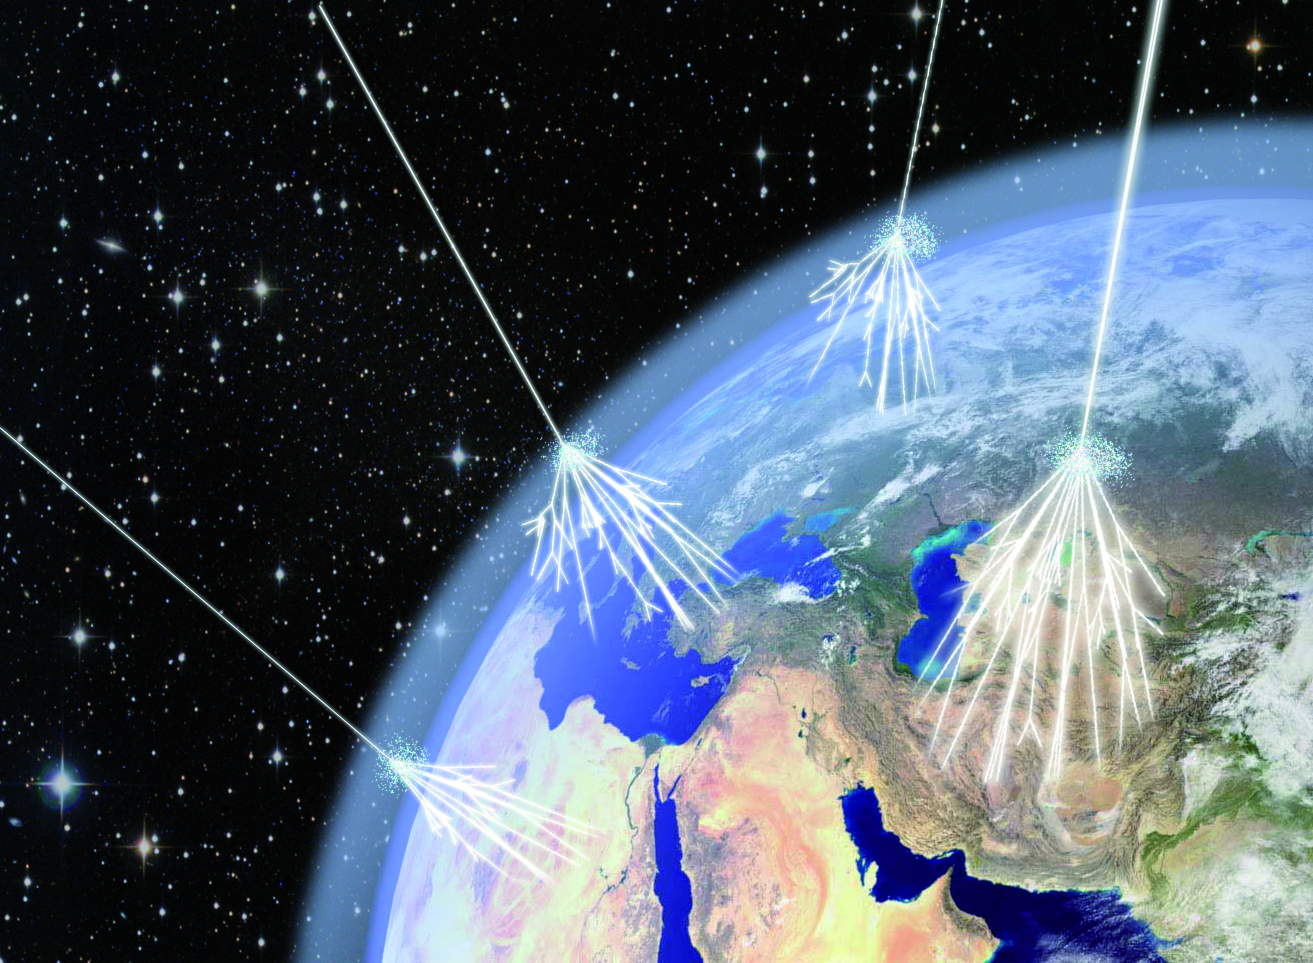
\includegraphics[width=\textwidth]{graphics/cosmicRays/cosmicRays.jpg}
	\end{minipage}
	\begin{minipage}[d]{0.49 \textwidth}
		  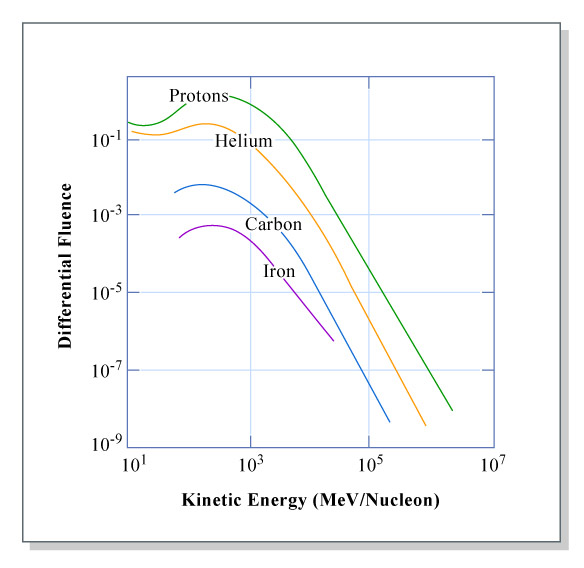
\includegraphics[width=\textwidth]{graphics/cosmicRays/energySpectrum.jpg}
	\end{minipage}
	\caption[Cosmic ray composition]{On the left, an artistic impression of various cosmic rays hitting the atmosphere \cite{airShower}. On the right, the measured composition for cosmic nuclei is shown: on top, the lightest particle, the proton. further down, all with orders of magnitude smaller rates, heavier ions, figure from \cite{highEnergyCosmicRays}.}
	\label{fig:Introduction:sec:CosmicRays}
    \end{figure}
    \todo{insert right side graphic from TODOR}
    By different forms of interaction, roughly dividable into the three groups of electromagnetic, inelastic hadronic and nuclear phenomena, secondary particles are created \cite{highEnergyCosmicRays, Grupen}. 
    \begin{itemize}
    	\item {\bf Nuclear fragmentation}\\
    	For very high energy primary particles above the separation energy $E_s$ according to 
		\begin{equation}
			E_s \simeq E_b(N,Z) - E_b(N_F, Z_F) - E_b(N - N_F, N - Z_F) - \frac{Z_F(Z -Z_F)}{(A-F)^{1/3}}
		\end{equation}
		it is possible to fragment a nucleous. The first three terms describe the binding energies of the nuclei involved, the last term accounts for the coulomb barrier. Of course, especially for higher order nuclei, more effects become relevant and one has to rely on empirical descriptions of the problem.
		\item{\bf Inelastic hadronic interaction}\\
		For high energies, quantum chromo dynamics describe the interactions of particles pretty well, while for energies below \SI{1}{\TeV} one has to rely on phenomenological descriptions. These interactions are prominent in the production of secondary particles like pions or kaons.
		
		\item{\bf Electromagnetic interaction}\\
		The electromagnetic component is the main interaction channel for lighter, charged particles like muons or electrons but also for photons. As the propagation of muons is especially important here, these interactions will be described in some more detail.
	
	
	\begin{itemize}
		\item {\bf Coulomb scattering}\\
		If one charged particle passes another, it is deflected in its field according to
		\begin{equation}
			\tan{\frac{\theta}{2}} = \frac{zZe^2}{Mv^2b}
		\end{equation}
		\item{\bf Ionization losses}\\
		Through ionization and excitation of molecules, incident particles loose energy in a medium, in this case the atmosphere, according to
		\begin{equation}
			\frac{dE}{dx} = -\frac{N_AZ}{A}\frac{2\pi\left(ze^2\right)^2}{M'nu^2}\left[\ln{\frac{2Mv^2\gamma^2}W{I^2}}-2\beta^2\right]
		\end{equation}
		$Z$ is the atomic, $A$ the mass number of the medium, $I$ the average ionization potential. $N_a$ is Avogadro's number, $ze$ the particle charge, $v$ its velocity and $M$ its mass. $\beta = v/c$ and $\gamma = 1/\sqrt{1-/\beta^2}$ and $W$ the maximum energy deposit \cite{Hayakawa}.\\
		This is the effect used for muon detection in the KATRIN experiment, see \ref{ch:The muon detection system}.
		
		\item{\bf Compton scattering \& inverse compton effect}\\
		Compton scattering is the photonic counterpart to ionization by charged particles. In the process, a photon interacts with bound electrons and excites or ionizes the corresponding atom. In the process the photon looses energy shifting it towards longer wavelengths.\\
		The inverse compton effect, as the name suggests, describes a photon gaining energy from an atom's hull electron.
		
		\item{\bf Bremsstrahlung \& synchrotron radiation}\\
		When charged particles are deflected in electric fields, photons are emitted and the particle looses energy. The same is applicable for magnetic fields, where the effect is called synchrotron radiation and a time dependent energy loss occurs. The total energy loss for electric fields can be described by
		\begin{equation}
			\frac{dE}{dx} = \frac{4N_AZ^2}{A}\alpha r_e^2 E  \ln{\left(183 Z^{1/3}\right)} = \frac{E}{X_0}
		\end{equation}
		where the radiation length has been introduced to describe the average matter necessary for a particular Energy loss.
		
		\item{\bf Electron-positron creation}\\
		A photon of sufficient energy (2 x \SI{511}{\kilo\electronvolt}) can create a electron-positron pair either in the field of an atom's electron hull or in the field of its core. With higher energies, other particles can be created considering the known conservation laws. 
		This proccess can be seen as the inverse bremsstrahlung, assuming the outgoing anti-particle to be its time inverted particle. The energy loss can be described similarly and scales with the incident particle's energy linearly.

		\item{\bf Cherenkov radiation}\\
		Much lower amounts of energy are lost in the creation of cherenkov light. The process is particularly important though as it makes for easily detectable particle indicators. Cherenkov radiation occurs when particles move through matter at speeds above the phase velocity of light $c/n$ for a refractive index $n$. As the atmospheric refractive index is only slightly above 1, particles need to be super-relativistic to emit cherenkov light. 		
    \end{itemize}
    \end{itemize}
	After cascading mostly through multiple intermediate particles, at sea level about \SI{80}{\percent} of the cosmic particles are muons. These are super-relativistic due to their small masses though high energies. Even at these high speeds, the muons' average decay time of around \SI{2.2}{\micro\second} \cite{muonLifetime} is too small for many muons to reach the earth's surface from our reference frame's point of view. In the most common production height of \SI{2}{\kilo\meter} \cite{muonProductionHeight}, the non relativistic time of flight for a \SI{90}{\percent} speed of light particle would be
    \begin{equation}
	t_{class} = \SI{2}{\kilo\meter} / 0.9\cdot c = 
    \end{equation}
    meaning only time dilation from special relativity makes the muon flux as large as it is:
    \begin{equation}
    	t_{rel} = t_{class} / \sqrt{1-0.9^2}
    \end{equation}
    which, from our reference frame, prolongs the lifetime by a factor of around 5, being already enough to reach the surface from heights of \SI{3}{\kilo\meter}. Most muons have even higher energies, making it possible for them to reach surface from greater heights and under non perpendicular angles towards it.
    For KATRIN, this poses a problem. A smaller flux would be advantageous, as muons may cause emission of electrons from the spectrometer vessels surface. Shielding against muons is difficult as it requires thick layers of dense matter due to the muons high energies and the low deposition in matter in relations to those.
    The fluctuation of energy deposition of a charged particle as the muon in matter can be described by the landau distribution that is parametrized as follows \cite{Grupen}.
    \begin{equation}
    	L(E) = \frac{1}{2\pi}\exp{\left\{-\frac{1}{2}\left(E- \hat E + \exp \left(-(E-\hat E)\right)\right)\right\}}
    \end{equation}
	$\hat E$ is the most probable energy deposition value. The analytic distribution is shown in figure \ref{fig:Introduction:landauDistribution}. The muon modules show that distribution as expected, see \ref{ch:The muon detection system} for details.
	\begin{figure}[H]
	\centering
		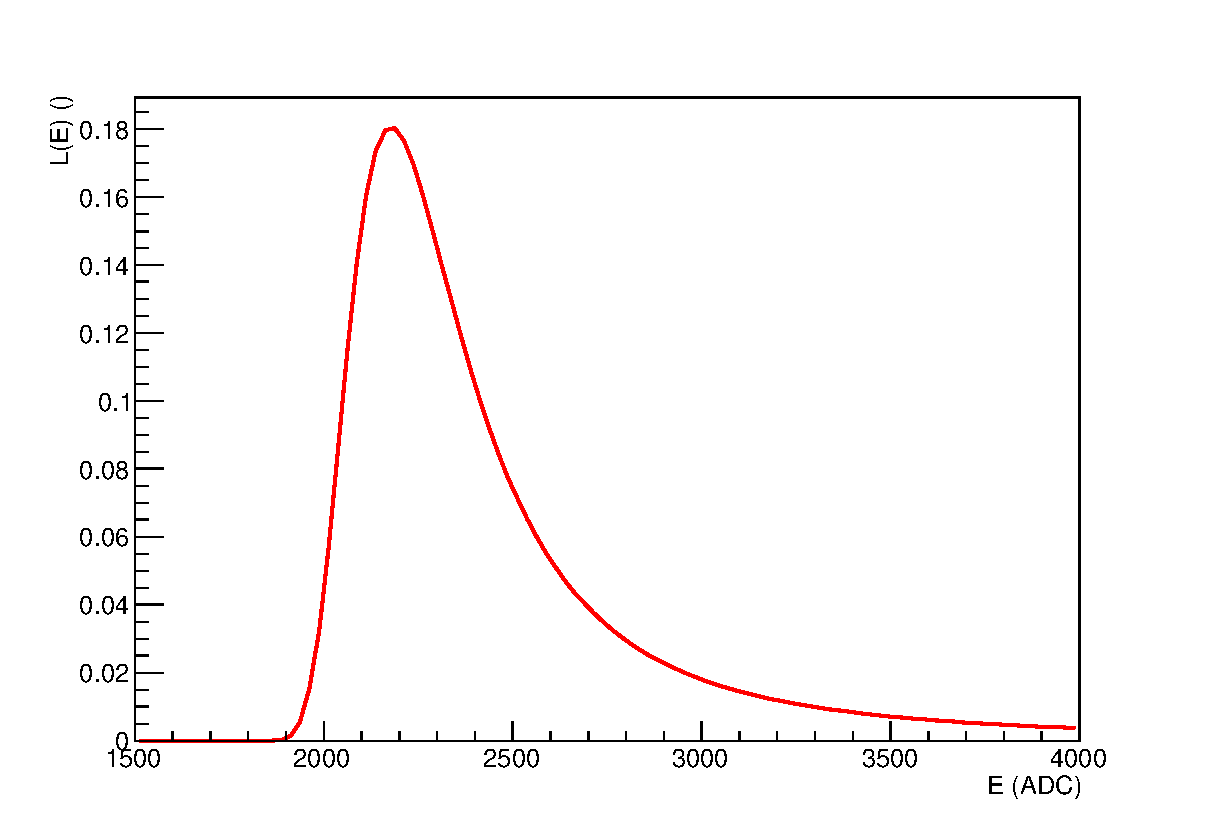
\includegraphics[width = 0.9 \textwidth]{graphics/cosmicRays/TMathLandauRoot.eps}
		\caption[Landau distribution]{Analytic landau distribution as implemented in the ROOT software. $\hat E$ was set to 1200.}
		\label{fig:Introduction:landauDistribution}
	\end{figure}

    
   